\documentclass[10pt]{amsart}
\usepackage[margin=1.4in]{geometry}
\usepackage{amssymb,amsmath,enumitem,url}
\usepackage{graphicx,subfig}
\graphicspath{ {./images/} }

\newcommand{\D}{\mathrm{d}}
\newcommand{\I}{\mathrm{i}}
\DeclareMathOperator{\E}{e}
\DeclareMathOperator{\OO}{O}
\DeclareMathOperator{\oo}{o}
\DeclareMathOperator{\erfc}{erfc}
\DeclareMathOperator{\real}{Re}
\DeclareMathOperator{\imag}{Im}
\usepackage{tikz}
\usepackage[framemethod=tikz]{mdframed}
\theoremstyle{nonumberplain}

\mdtheorem[innertopmargin=-5pt]{sol}{Solution}
%\newmdtheoremenv[innertopmargin=-5pt]{sol}{Solution}

\begin{document}
\pagestyle{empty}

\newcommand{\mline}{\vspace{.2in}\hrule\vspace{.2in}}

\noindent
\text{Hunter Lybbert} \\
\text{Student ID: 2426454} \\
\text{01-16-25} \\
\text{AMATH 502} \\
% header containing your name, student number, due date, course, and the homework number as a title.

\title{\bf {Homework 1} }


\maketitle
\noindent
Exercises come from \textit{Nonlinear Dynamics and Chaos by Steven H. Strogatz}
\mline
\begin{enumerate}[label={\bf {\arabic*}:}]
\item 2.2.3 \\
\textit{Solution:}
Looking closely at the DS $\dot x = x - x^3$, we can recognize there are three fixed points at $x^* = -1, 0, 1$.
Now we can look at the plots in Figure \ref{fig:f1}, to identify that $x^* = -1, 1$ are stable fixed points and $x^* = 0$ is unstable.
\begin{figure}[h]
	\centering
	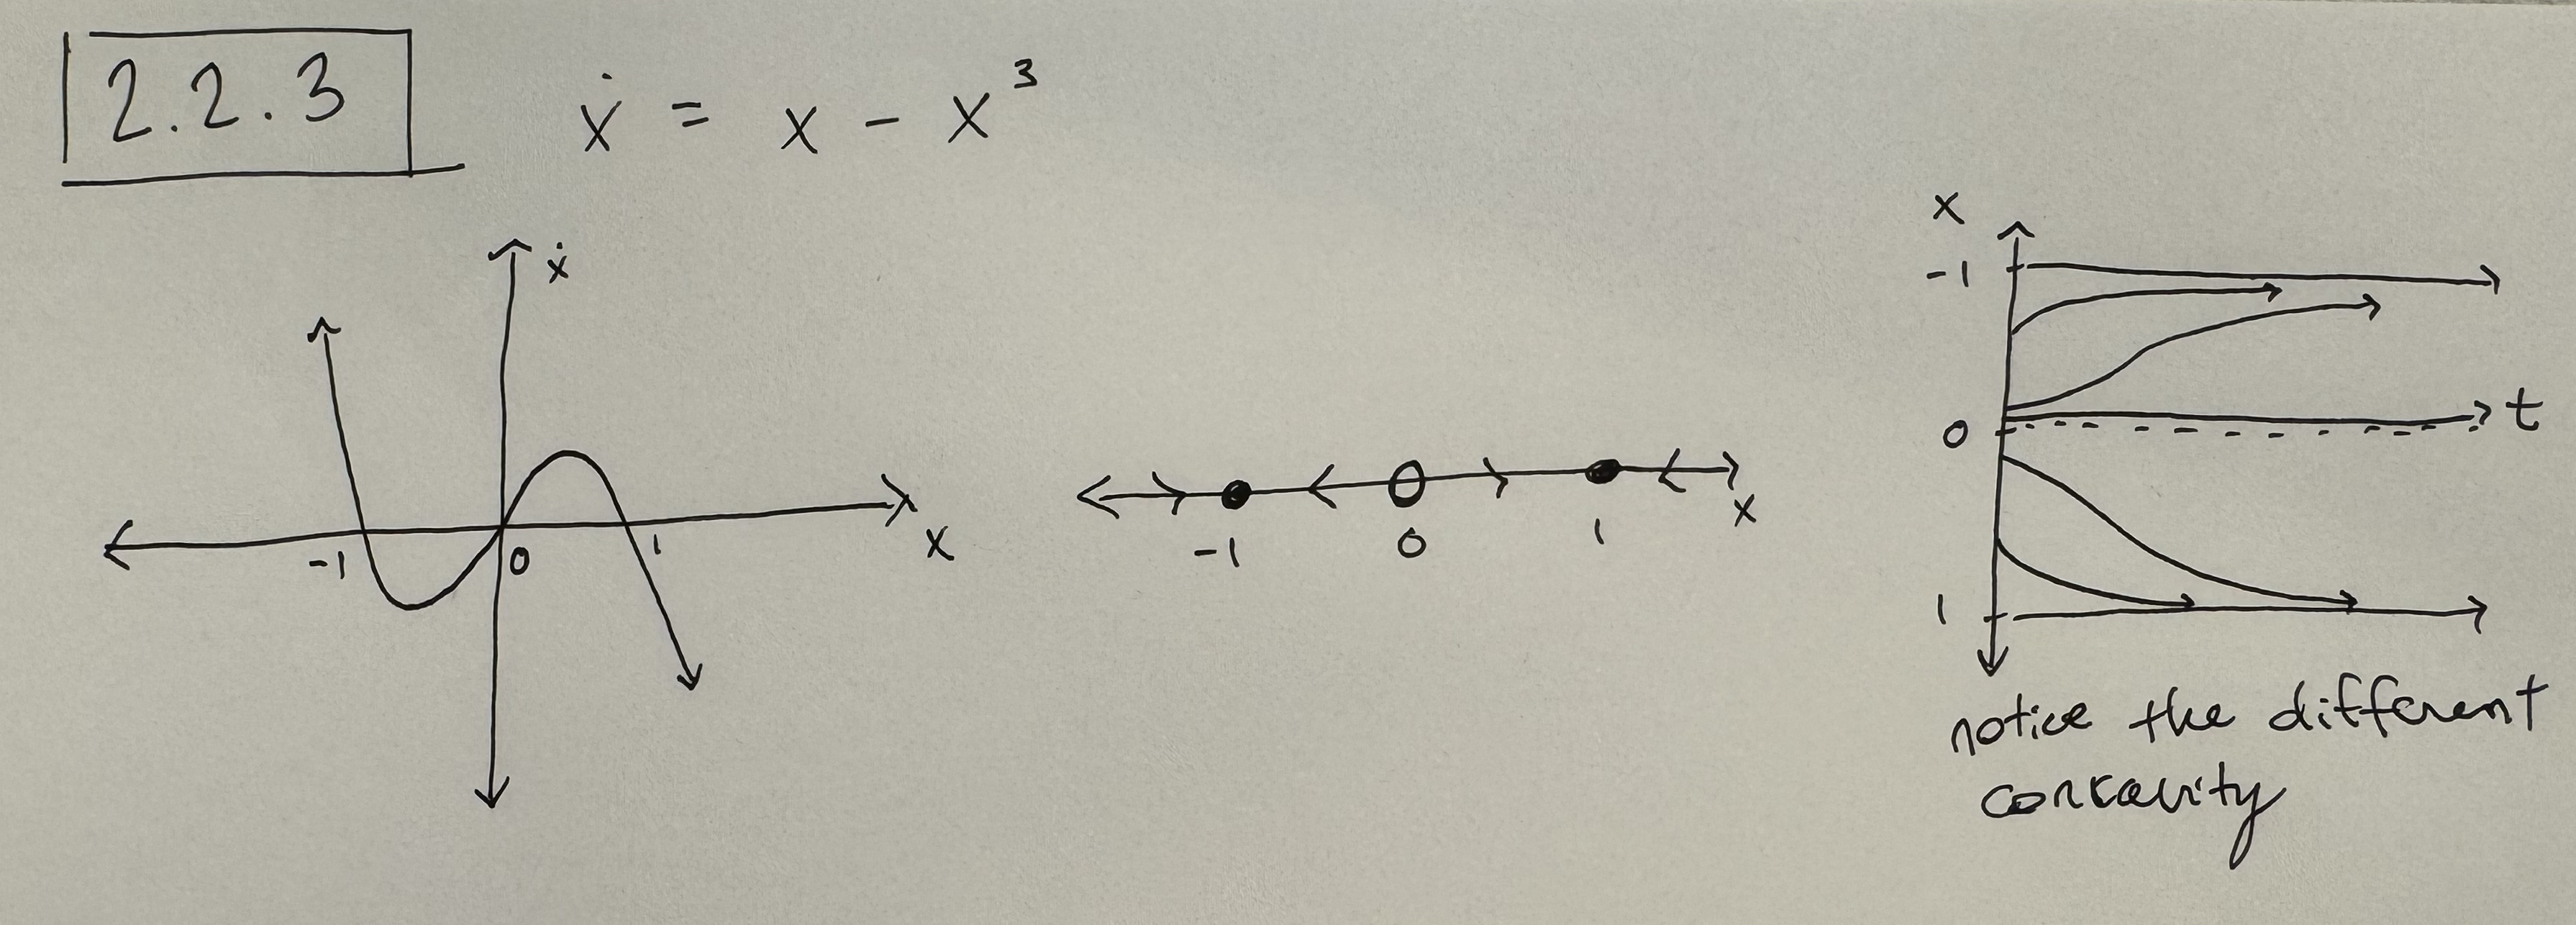
\includegraphics[width=1\textwidth]{2_2_3.png}
 	\caption{We have sketched the vector field on the real line, identified all three fixed points, classified their stability and sketched the $x(t)$ for different initial conditions.}\label{fig:f1}
\end{figure}

\qed \\

\newpage

\item 2.2.7 \\
\textit{Solution:} Looking at the DS $\dot x = \E^x - \cos x$ is tricky so let's plot each of $\E^x$ and $\cos x$ on the same plot to determine where the fixed points are and what their stability is.
\begin{figure}[h]
	\centering
	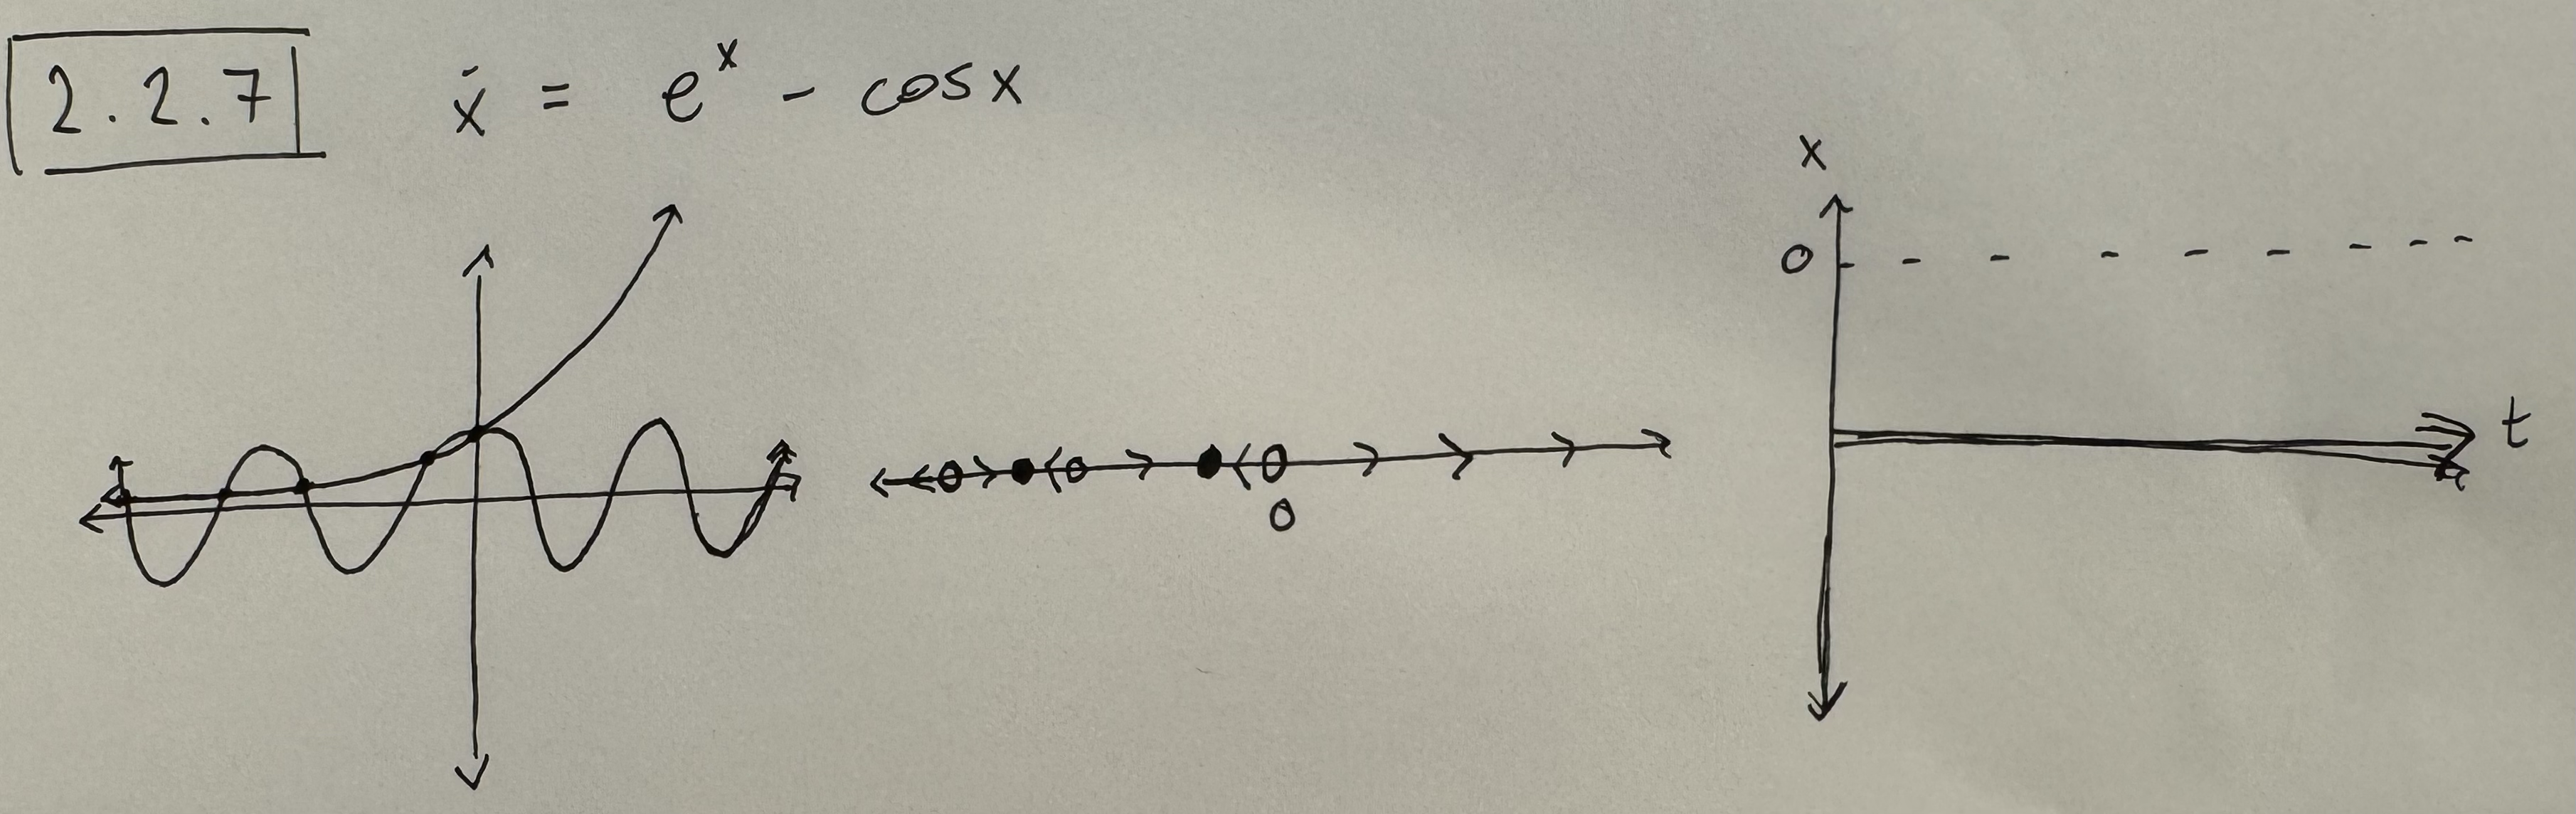
\includegraphics[width=1\textwidth]{2_2_7.png}
 	\caption{We have sketched the vector field on the real line, identified the approximate location of all the fixed points,  and classified their stability (which is alternating stable and unstable) sketched the $x(t)$ for different initial conditions.}\label{fig:f2}
\end{figure}

\qed \\

\newpage

\item 2.2.8 \\
\textit{Solution:} \\
\textbf{TODO} \\

\item 2.2.10 \\
\textit{Solution:} \\
\textbf{TODO} \\

\item 2.2.13 (a,b,c,d) \\
\begin{enumerate}
\item $m \dot v = mg - kv^2$ with initial condition $v(0) = 0$ \\

\noindent
\textit{Solution:} \\
Let's begin by dividing by $m$ and factoring out a $g$ term.
\begin{align*}
m \dot v &= mg - kv^2 \\
\dot v &= g - \frac{kv^2}{m} \\
\dot v &= g\left( 1 - \frac{kv^2}{gm}\right).
\end{align*}
Now rewriting $\dot v$ as the derivative of $v$ with respect to $t$ we have
\begin{align*}
\frac{\D v}{\D t} &= g\left( 1 - \frac{kv^2}{gm}\right) \\
\frac{1}{\left( 1 - \frac{kv^2}{gm}\right)}\D v &= g \D t \\
\int \frac{1}{\left( 1 - \sqrt{\frac{k}{gm}}v\right)\left( 1 + \sqrt{\frac{k}{gm}}v\right)}\D v &= \int g \D t.
\end{align*}
Now, we can do partial fractions on the left and integrate both sides
\begin{align*}
\int \frac{1}{\left( 1 - \sqrt{\frac{k}{gm}}v\right)\left( 1 + \sqrt{\frac{k}{gm}}v\right)}\D v &= \int g \D t \\
\int \frac{1/2}{\left( 1 - \sqrt{\frac{k}{gm}}v\right)}\D v
	+ \int \frac{1/2}{\left( 1 + \sqrt{\frac{k}{gm}}v\right)}\D v
	 &= g t + C \\
- \frac 1 2 \sqrt{\frac {gm}{k}}\log\left( 1 - \sqrt{\frac{k}{gm}}v\right)
	+ \frac 1 2 \sqrt{\frac {gm}{k}}\log\left( 1 + \sqrt{\frac{k}{gm}}v\right)
	 &= g t + C \\
\frac 1 2 \sqrt{\frac {gm}{k}}\Bigg( \log \left( 1 + \sqrt{k/(gm)} \: v\right) 
	- \log \left( 1 - \sqrt{k/(gm)} \: v\right) \Bigg)
	 &= g t + C
\end{align*}
Interesting ... now I need to input the initial condition \\
\begin{align*}
\frac 1 2 \sqrt{\frac {gm}{k}}\Bigg( \log \left( 1 + \sqrt{k/(gm)} \: 0\right) 
	- \log \left( 1 - \sqrt{k/(gm)} \: 0\right) \Bigg)
	 &= g 0 + C \\
\frac 1 2 \sqrt{\frac {gm}{k}}\Bigg( \log \left( 1 \right) 
	- \log \left( 1 \right) \Bigg) &= C \\
	0 &= C.
\end{align*}
Plugging this in and simplifying we have
\begin{align*}
\frac 1 2 \sqrt{\frac {gm}{k}}\Bigg( \log \left( 1 + \sqrt{k/(gm)} \: v\right) 
	- \log \left( 1 - \sqrt{k/(gm)} \: v\right) \Bigg)
	 &= g t \\
\log \left( \frac {1 + \sqrt{k/(gm)} \: v}{1 - \sqrt{k/(gm)} \: v}\right) 
	 &= 2 g t \sqrt{k/(gm)}.
\end{align*}
Now we can exponentiate and solve for $v$
\begin{align*}
\frac {1 + \sqrt{k/(gm)} \: v}{1 - \sqrt{k/(gm)} \: v}
	 &= \E^{2 g t \sqrt{k/(gm)}} \\
1 + \sqrt{k/(gm)} \: v
	 &= \E^{2 g t \sqrt{k/(gm)}}(1 - \sqrt{k/(gm)} \: v) \\
1 + \sqrt{k/(gm)} \: v 
	 &= \E^{2 g t \sqrt{k/(gm)}} - \sqrt{k/(gm)} \: v \E^{2 g t \sqrt{k/(gm)}} \\
\sqrt{k/(gm)} \: v +  \sqrt{k/(gm)} \: v \E^{2 g t \sqrt{k/(gm)}}
	 &= \E^{2 g t \sqrt{k/(gm)}} - 1 \\
v &= \frac {\E^{2 g t \sqrt{k/(gm)}} - 1}{\sqrt{k/(gm)} +  \sqrt{k/(gm)} \E^{2 g t \sqrt{k/(gm)}}}.
\end{align*}
Some final simplifications gives us
\begin{align*}
v &= \frac 1 {\sqrt{k/(gm)}}\frac {\E^{2 g t \sqrt{k/(gm)}} - 1}{1 +  \E^{2 g t \sqrt{k/(gm)}}} \\
v &= \sqrt{\frac {gm}{k}} \left( \frac {\E^{2 g t \sqrt{k/(gm)}} - 1}{\E^{2 g t \sqrt{k/(gm)}}+ 1} \right).
\end{align*}
Therefore our final analytical solution is 
$$
v = \sqrt{\frac {gm}{k}} \left( \frac {\E^{2 g t \sqrt{k/(gm)}} - 1}{\E^{2 g t \sqrt{k/(gm)}}+ 1} \right).
$$
\qed \\

\item Determine the limit of $v(t)$ as $t\rightarrow \infty$.
We will need to utilize L'Hôpital's rule since the numerator and the denominator go to infinity.
\begin{align*}
\lim_{t\rightarrow \infty} \sqrt{\frac {gm}{k}} \left( \frac {\E^{2 g t \sqrt{k/(gm)}} - 1}{\E^{2 g t \sqrt{k/(gm)}}+ 1} \right)
	&= \lim_{t\rightarrow \infty} \sqrt{\frac {gm}{k}} \left( \frac {2 g t \sqrt{k/(gm)}\E^{2 g t \sqrt{k/(gm)}}}{2 g t \sqrt{k/(gm)}\E^{2 g t \sqrt{k/(gm)}}} \right) \\
	&= \lim_{t\rightarrow \infty} \sqrt{\frac {gm}{k}} \\
	&= \sqrt{\frac {gm}{k}}.
\end{align*}
Therefore, the terminal velocity is $\sqrt{\frac {gm}{k}}$. \\
\qed \\

\item \textbf{TODO:} insert pictures.
\item 
\end{enumerate}

\item 2.3.2 \\
\textit{Solution:} \\
\textbf{TODO} \\

\item 2.3.6 \\
\textit{Solution:} \\
\textbf{TODO} \\

\item 2.4.7 \\
\textit{Solution:} \\
\textbf{TODO} \\

\end{enumerate}

\end{document}

%%% Local Variables:
%%% mode: latex
%%% TeX-master: t
%%% End:
